\documentclass[12pt,letterpaper]{exam}
\usepackage[lmargin=1in,rmargin=1in,tmargin=1in,bmargin=1in]{geometry}
\usepackage{../style/exams}

% -------------------
% Course & Exam Information
% -------------------
\newcommand{\course}{MAT 104: Exam 1}
\newcommand{\term}{Spring --- 2024}
\newcommand{\examdate}{02/22/2024}
\newcommand{\timelimit}{85 Minutes}

\setbool{hideans}{true} % Student: True; Instructor: False


% -------------------
% Content
% -------------------
\begin{document}

\examtitle
\instructions{Write your name on the appropriate line on the exam cover sheet. This exam contains \numpages\ pages (including this cover page) and \numquestions\ questions. Check that you have every page of the exam. Answer the questions in the spaces provided on the question sheets. Be sure to answer every part of each question and show all your work. If you run out of room for an answer, continue on the back of the page --- being sure to indicate the problem number.} 
\scores
\bottomline
\newpage


% -------------------
% Questions
% -------------------
\begin{questions}

% Question 1
\newpage
\question[10] Showing all your work and simplifying as much as possible, compute the exact values of the following:
	\begin{enumerate}[(a)]
	\item $6 \div 2(1 + 2)$ \par\vspace{0.3cm}
	\item $\dfrac{-3 - 5(-1)^2 + 12}{-6 - (-8)}$ \par\vspace{0.3cm}
	\item  $(1 - 3)^3 \cdot 4 (7 - 2 \cdot 3)$
	\end{enumerate}



% Question 2
\newpage
\question[10] Consider the points $A(-7, 6)$, $B(4, -8)$, and $C(5, 1)$. 

\begin{enumerate}[(a)]
\item Plot the points on the graph below, be sure to label each point. 
\item Fill in the missing entries to the non-greyed portion of the chart below. 
\end{enumerate}
	\[
	\fbox{
	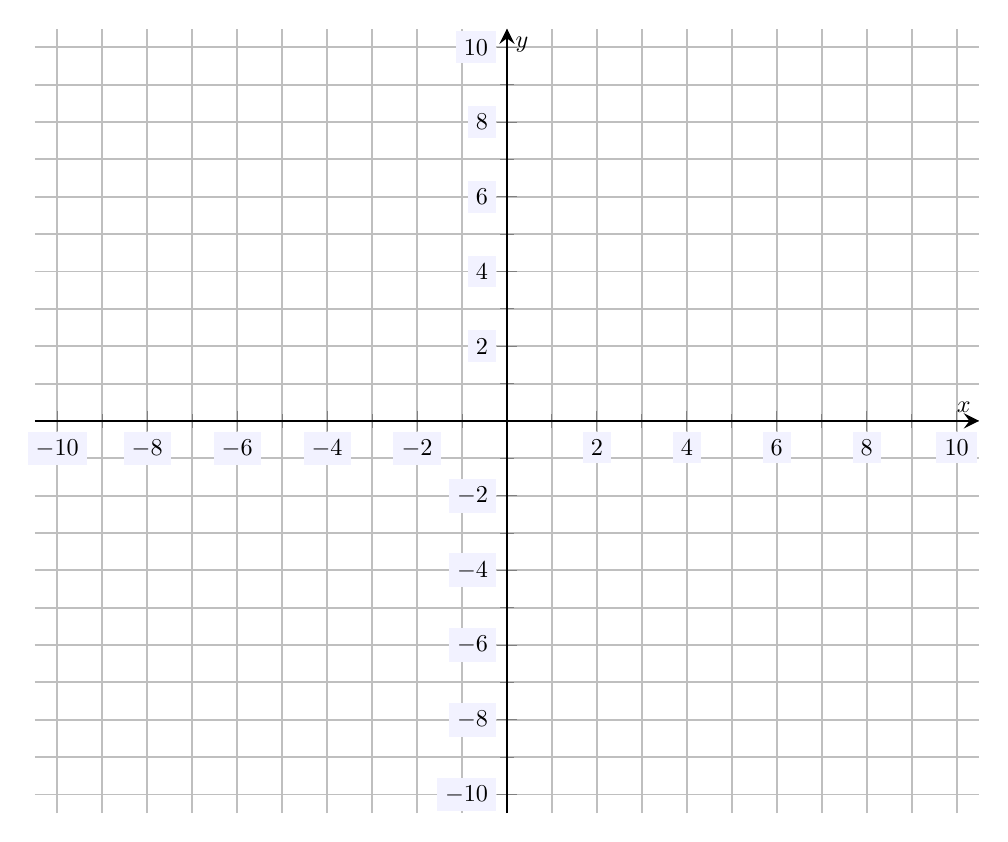
\begin{tikzpicture}[scale=1.75,every node/.style={scale=0.5}]
	\begin{axis}[
	grid=both,
	axis lines=middle,
	ticklabel style={fill=blue!5!white},
	xmin= -10.5, xmax=10.5,
	ymin= -10.5, ymax=10.5,
	xtick={-10,-8,-6,-4,-2,0,2,4,6,8,10},
	ytick={-10,-8,-6,-4,-2,0,2,4,6,8,10},
	minor tick = {-10,-9,...,10},
	xlabel=\(x\),ylabel=\(y\),
	]
	\end{axis}
	\end{tikzpicture}
	}
	\] 

\begingroup
\renewcommand*{\arraystretch}{2}
\begin{table}[ht]
\begin{tabular}{| >{\centering\arraybackslash}m{1.5cm} | >{\centering\arraybackslash}m{2.5cm} | >{\centering\arraybackslash}m{3.5cm} | >{\centering\arraybackslash}m{3.5cm} | >{\centering\arraybackslash}m{3.5cm} |}
\hline
 & Quadrant & Distance to $x$-axis & Distance to $y$-axis & Distance to origin \\ \hline
Point $A$ &  & \cellcolor[HTML]{9B9B9B} &  & \cellcolor[HTML]{9B9B9B} \\ \hline
Point $B$ &  &  & \cellcolor[HTML]{9B9B9B} & \cellcolor[HTML]{9B9B9B} \\ \hline
Point $C$ &  & \cellcolor[HTML]{9B9B9B} & \cellcolor[HTML]{9B9B9B} &  \\ \hline
\end{tabular}
\end{table}
\endgroup
	
	

% Question 3
\newpage
\question[10] Consider the quadratic function $f(x)= x^2 - 3x + 4$ and the linear function $\ell(x)= 7 - 2x$. Let $\mathcal{I}$ be the interval $\mathcal{I}= [-1, 3]$.
	\begin{enumerate}[(a)]
	\item Find the average rate of change for $f(x)$ on $\mathcal{I}$.
	\item What is the slope of the secant line to $f(x)$ using the points on the graph of $f(x)$ where $x= -1$ and $x= 3$?
	\item Without explicitly calculating the average rate of change, what is the average rate of change for $\ell(x)$ on $\mathcal{I}$?
	\end{enumerate}



% Question 4
\newpage
\question[10] Consider the linear function $\ell(x)= \frac{2}{3}\, x + 4$.
	\begin{enumerate}[(a)]
	\item Find the slope of $\ell(x)$.
	\item Find the $y$-intercept of $\ell(x)$.
	\item Sketch $\ell(x)$ on the graph below as accurately as possible.
	\item Find the $x$-intercept of $\ell(x)$. 
	\end{enumerate}

	\vfill

	\[
	\fbox{
	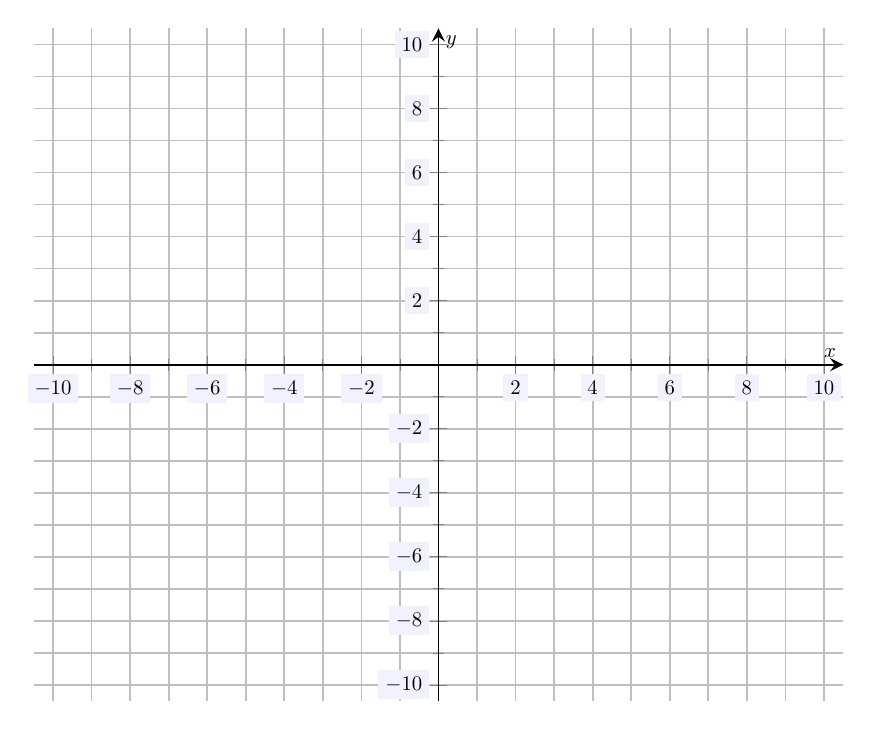
\begin{tikzpicture}[scale=1.5,every node/.style={scale=0.5}]
	\begin{axis}[
	grid=both,
	axis lines=middle,
	ticklabel style={fill=blue!5!white},
	xmin= -10.5, xmax=10.5,
	ymin= -10.5, ymax=10.5,
	xtick={-10,-8,-6,-4,-2,0,2,4,6,8,10},
	ytick={-10,-8,-6,-4,-2,0,2,4,6,8,10},
	minor tick = {-10,-9,...,10},
	xlabel=\(x\),ylabel=\(y\),
	]
	\end{axis}
	\end{tikzpicture}
	}
	\] 



% Question 5
\newpage
\question[10] Otto Partze owns an automotive parts and repair shop. When a customer brings in a car for service, the amount Otto charges for service is given by $C(t)= 81t + 45$, where $t$ is the number of hours of work done. 
	\begin{enumerate}[(a)]
	\item Find and interpret the slope of $C(t)$. Be sure to include any units.
	\item Find and interpret the $y$-intercept of $C(t)$. Be sure to include any units. 
	\item Find the cost of 90~minutes of service. 
	\end{enumerate}



% Question 6
\newpage
\question[10] Jenna Rossity purchased a new 85" TV for her nephew. The TV cost \$1,599.99. As with any new electronics, the TV depreciates in value by \$372 per year. 
	\begin{enumerate}[(a)]
	\item Find a linear function that gives the resale value of the TV $t$~years from now. 
	\item Find how long until the TV has no resale value. 
	\end{enumerate}



% Question 7
\newpage
\question[10] Showing all your work, find the equation of line given in the graph below. If you use any points on the line, be sure that any points you use are \textit{exactly} on the line. 
	\[
	\fbox{
	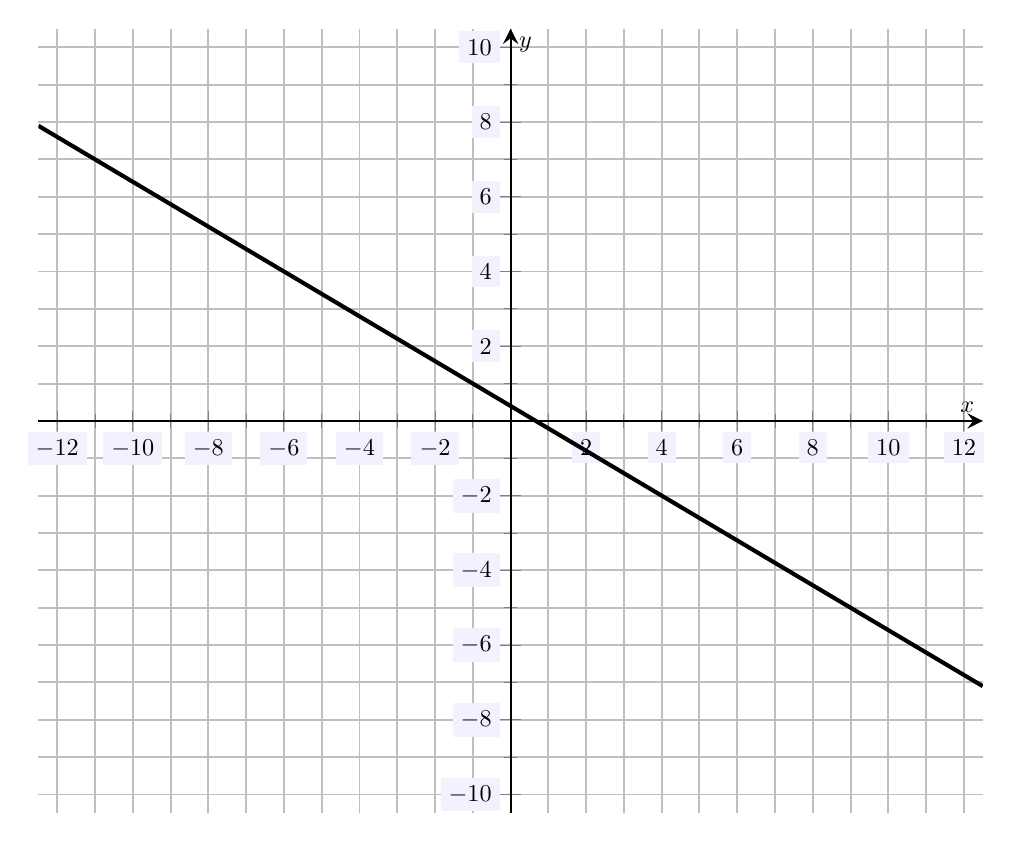
\begin{tikzpicture}[scale=1.75,every node/.style={scale=0.5}]
	\begin{axis}[
	grid=both,
	axis lines=middle,
	ticklabel style={fill=blue!5!white},
	xmin= -12.5, xmax=12.5,
	ymin= -10.5, ymax=10.5,
	xtick={-12,-10,...,12},
	ytick={-12,-10,...,12},
	minor tick = {-12,-11,...,12},
	xlabel=\(x\),ylabel=\(y\),
	]
	\addplot[line width=0.03cm,domain=-12.5:12.5] ({x},{(2 - 3*x)/5});
	\end{axis}
	\end{tikzpicture}
	}
	\] 



% Question 8
\newpage
\question[10] Find the exact equation of the line with $x$-intercept $7$ and $y$-intercept $-4$. Express your answer in slope-intercept form. 



% Question 9
\newpage
\question[10] Find the exact equation of the line parallel to the line $y= 9x - 16$ that contains the point $(-1, 7)$. Express your answer in point-slope form. 



% Question 10
\newpage
\question[10] Find the exact equation of the line perpendicular to $y= \dfrac{1 - 4x}{2}$ that passes through the $x$-intercept of $f(x)= 4(1 - 3x)$. 


\end{questions}
\end{document}